Kapitulu honetan txantiloiaren erabilera landuko da. Txantiloiko berezitasunaz gain, \LaTeX eko elementu nagusiak ere aztertuko dira. 

\section{Txantiloia}

Txantiloian zenbait fitxategi daude. Fitxategi nagusia \texttt{main.tex} izenkoa da. Horrez gain badaude beste fitxategi batzuk \texttt{config} direktorioan. Printzipioz, fitxategi horiek ez dira ikutu behar.

Fitxategi nagusian zenbait atal konfiguratu behar dira.

Lehenik eta behin, txantiloiak \texttt{memoir} estiloa erabiltzen du oinarritzat. Beraz, estilo horretan dauden aukera guztiak erabili daitezke. Gehienbat, kapituluen itxura alda daiteke estiloak erabiliz. Horretarako, \texttt{main.tex} fitxategiaren hasieran dagoen \texttt{chapterstyle} komandoan estiloa aldatu behar da. Hauek dira aukerak:
\begin{itemize}
	\item bianchi
	\item bringhurst
	\item brotherton
	\item chappell
	\item crosshead
	\item culver
	\item dash
	\item demo2
	\item demo3
	\item dowding
	\item \textbf{ell}
	\item ger
	\item komalike
	\item lyhne
	\item madsen
	\item ntglike
	\item pedersen
	\item \textbf{southall}
	\item \textbf{tandh}
	\item thatcher
	\item veelo
	\item \textbf{verville}
	\item \textbf{wilsondob}
\end{itemize}

Beltzen markatuta dauden estiloetan kapitulu hitza ez da erabiltzen eta, hortaz, euskarazko memorientzako bereziki erabilgarriak dira.

\subsection{Proiektuaren informazioa}

Estiloa definitu ondoren informazio orokorra betetzeko komandoak agertzen dira. Egilearen izena, proiektuaren izenburua, zuzendarien izenak eta dokumentuaren data.

Informazio hori eta gero titulazioarena agertzen da. Horretarako \texttt{ikasketak} eta \texttt{espezialitatea} komandoak definitu behar dira, dagokien aukera deskomentatuz eta beste gainontzekoak komentatuz. Espezialitatea bakarrik Informatika Ingeniaritzako Gradurako da.

\subsection{Dokumentuaren hizkuntza}

Dokumentua euskaraz, gazteleraz edo ingelesez idatzi daiteke. Behar den bezala konfiguratzeko \texttt{main.tex} fitxategian hizkuntza definitu behar da, nahi den aukera deskomentatuz. Bakarrik aukera bat egon behar da deskomentatuta.

\begin{table}[t]
	\centering
	\begin{tabular}{l|llll}
		Y & A & B & C & D\\
		\hline
		y1 & a1 & b1 & c1 & d1\\
		y2 & a2 & b2 & c2 & d2\\
	\end{tabular}
	\caption {Taularen adibidea}\label{tab:adibidea}
\end{table}

\subsection{Dokumentuaren azala}

Bi aukera daude dokumentuaren azala sortzeko. Lehenengoa PDF bat txertatzea da. Defektuz \texttt{cover.pdf} dokumentua txertatzen da. Aukera hau erabili nahi ez baduzu, \texttt{includepdf} komandoa komentatu behar duzu. 

Bigarren aukera \texttt{cover\_XXX} fitxategiak erabiltzea da. Hiru daude, bat Informatika Ingeniaritzako Gradurako, bat Adimen Artifizialeko Gradurako eta beste bat Master Amaierako Lanetarako. Erabili nahi dena deskomentatu behar da, besteak komentatuta mantenduz.

Erabili daiteke bata, bestea edo biak. \texttt{cover\_XXX} fitxategiekin agertzen den informazioa PDF formatuan dagoen azalan agertzen bada, horrekin nahikoa da. Bestela, informazioa bertan ez badago, biak sartu beharko dira.

\subsection{Dokumentuaren edukia}

Dokumentuaren edukia antolatzeko \texttt{chapters} karpetan dauden fitxategien bidez txertatzen da. \texttt{main.tex} dokumentuan kapituluen ideia garbia izatearren, kapituluen izenburua bertan definitzen da, nahiz eta kodea aipatutako karpetan dauden fitxategien bidez txertatu.


\section{Irudiak eta Taulak}

\begin{figure}[t]
	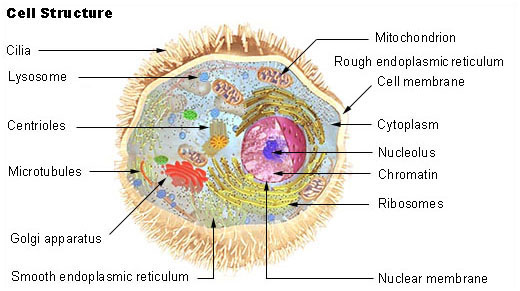
\includegraphics[width=0.5\textwidth]{figures/cell.jpg}
	\caption{Irudiaren adibidea}\label{fig:adibidea}
\end{figure}

Dokumentuaren itxura manentzearren gomendatzen da irudi eta taula guztiak goian edo behan jartzea. Horretarako \texttt{figure} eta \texttt{table} inguruneen \texttt{[t]} edo \texttt{[b]} aukerak erabili behar dira.

\ref{fig:adibidea} Irudian eta \ref{tab:adibidea} taulan adibideak ikusi daitezke. Kontutan izan behar da \LaTeX sistemak taulen eta irudien kokapen optimoak erabakitzen dituela. Esan bezala, komenigarria da irizpide bat jarraitzea (goian edo behan) eta hori mantentzea. Taula edo irudi baten kokapena orriz aldatzeko, kodearen kokapena aldatu behar da. Kontutan izan irudiaren edo taularen kodea ez daukala zergatik egon aipatzen den tokian, beti zenbakia erabiliz erreferentziatu behar da eta (ez ``goian'' edo ``behan'' terminoak erabiliz).

\section{Elementu matematikoak}

Elementu matematikoak \texttt{ifcommands} paketean definituta daude. \texttt{main.tex} fitxategiaren hasieran pakete hori kargatzen da eta bertan hizkuntza aukeratu daiteke.

Pakete horretan zenbait elementu definitzen dira. Jarraian zerrendatzen dira.

\begin{ifaxiom}
	Axiomaren adibidea
\end{ifaxiom}

\begin{iftheorem}
	Teoremaren adibidea
\end{iftheorem}

\begin{iflemma}
	Lemaren adibidea
\end{iflemma}

\begin{ifproposition}
	Proposizioaren adibidea
\end{ifproposition}

\begin{ifdefinition}
	Definizioaren adibidea
\end{ifdefinition}

\begin{ifexample}
	Adibidearen adibidea
\end{ifexample}

\begin{ifproblem}
	Problemaren adibidea
\end{ifproblem}

\begin{ifsolution}
	Soluzioaren adibidea
\end{ifsolution}

\begin{ifremark}
	Oharraren adibidea
\end{ifremark}

\begin{ifproof}{Frogaren izena}
	Frogaren adibidea \iqed
\end{ifproof}

\begin{ifalgorithm}[t]
	\begin{ifpseudo}{Algoritmoaren izena}
	\item	\In\ Sarrera
	\item	\Out\ Irteera
	\item	\For{1}{n}
	\item	\T{Lehenengo urratsa}
	\item	\EFor
	\item	\If\ baldintza \Then
	\item	\T{\While{beste baldintza}}
	\item	\TT{errepikatzeko urratsa}
	\item	\T{\Done}
	\item	\Else
	\item	\T{\Do}
	\item	\TT{\CFor elementu bakoitza}
	\item	\TTT{elementua prozesatu}
	\item	\TT{\EFor}
	\item	\T{\Until{hirugarren baldintza}}
	\item	\EIf
	\item	\WhileDo{azken baldintza}
	\item	\T{\If amaitu}
	\item	\TT{\Return}
	\item	\T{\EIf}
	\end{ifpseudo}
	\caption{Sasikodearen adibidea}\label{alg:adibidea}
\end{ifalgorithm}

Horrez gain, badago algoritmoak definitzeko bi ingurune, \texttt{ifalgorithm} eta \texttt{ifpseudo}. Posible da irudien eta taulen aurkibideaz gain, algoritmoen aurkibide bat sortzea. \ref{alg:adibidea} algoritmoan adibide bat ikusi daiteke.

Ekuazio matematikoei dagokienez, hauek testuan sartu daitezke: $X_n \geq 10$, edo testuarekin tartekatu:

\begin{eqnarray}
P(\Theta|D) = \frac{P(D|\Theta)P(\Theta)}{P(D)}\\
P(\Theta) \sim Beta(\alpha, \beta)
\end{eqnarray} 

Ekuazioak zenbatu gabe ere sar daitezke:

\begin{eqnarray*}
P(\Theta|D) = \frac{P(D|\Theta)P(\Theta)}{P(D)}\\
P(\Theta) \sim Beta(\alpha, \beta)
\end{eqnarray*} 

\section{Erreferentziak}

Bibliografia sartzeko BibTeX erabili behar da. Erreferntziak \texttt{erreferentziak.bib} fitxategian daude, eta textuan errferenziatzeko \texttt{cite} komandoa erabili behar da. Adibidez, \cite{Shahbaba2011} edo \cite{Efron1994, Rmanual, Subramanian2005gene}. Ez ahaztu erreferentzien informazio guztia sartzen (orrialdeak, urtea, etab.).

